% Fig. 1 -- key findings (IEEE double-column width, 7.16 in). Generated by gen_teaser.py
\documentclass[tikz,border=0pt]{standalone}
\usepackage[T1]{fontenc}
\usepackage{textcomp}
\usepackage{helvet}
\renewcommand{\familydefault}{\sfdefault}
\usetikzlibrary{arrows.meta,calc}
\definecolor{ink}{HTML}{1E2A36}
\definecolor{muted}{HTML}{5D6B7A}
\definecolor{faint}{HTML}{A3AFBB}
\definecolor{navy}{HTML}{1F4E79}
\definecolor{stagefill}{HTML}{F1F5F9}
\definecolor{grid}{HTML}{FFFFFF}
\definecolor{axis}{HTML}{8796A5}
\definecolor{rfifty}{HTML}{2878AD}
\definecolor{bfive}{HTML}{419A61}
\definecolor{isdnet}{HTML}{C54A43}
\definecolor{magnet}{HTML}{8964AB}
\definecolor{neg}{HTML}{F8EAE8}
\newcommand{\fs}{\fontsize{8}{9.4}\selectfont}
\newcommand{\fsb}{\fontsize{8}{9.4}\selectfont\bfseries}
\newcommand{\ftitle}{\fontsize{8.6}{10}\selectfont\bfseries}
\begin{document}
\frenchspacing\hyphenpenalty=10000\exhyphenpenalty=10000
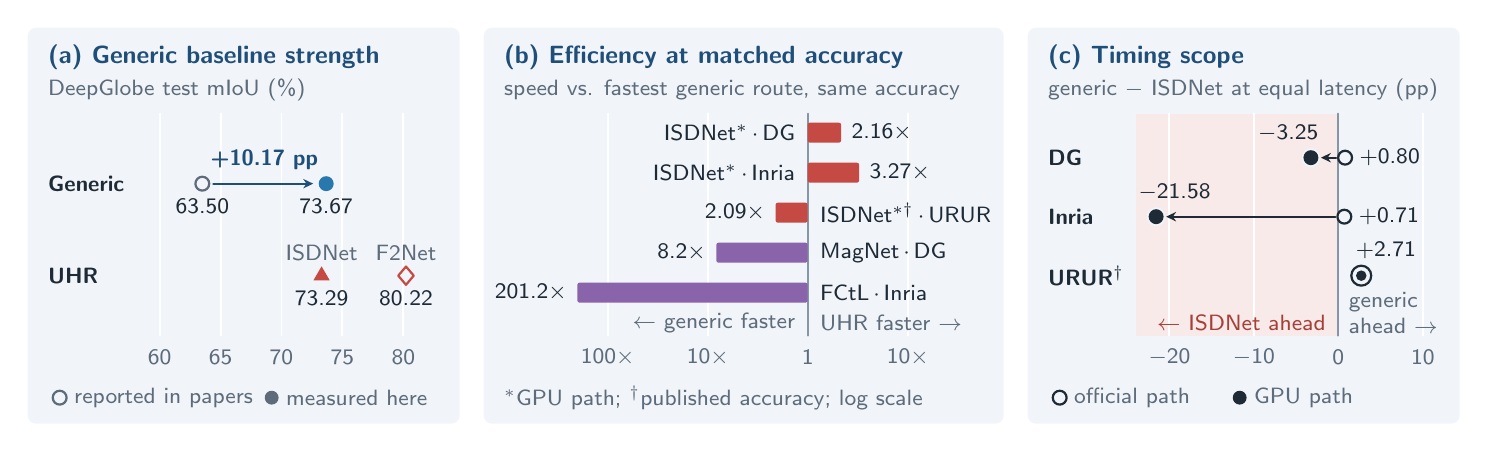
\begin{tikzpicture}[x=1in,y=1in,line join=round,line cap=round]
\useasboundingbox (0,0) rectangle (7.16,1.98);
\fill[stagefill, rounded corners=3pt] (0.0,0) rectangle (2.16,1.98);
\node[anchor=west, font=\ftitle, text=navy, inner sep=0pt] at (0.1,1.83) {(a) Generic baseline strength};
\node[anchor=west, font=\fs, text=muted, inner sep=0pt] at (0.1,1.67) {DeepGlobe test mIoU (\%)};
\draw[grid, line width=0.7pt] (0.6600,0.44) -- (0.6600,1.55);
\node[font=\fs, text=muted, inner sep=0pt] at (0.6600,0.33) {60};
\draw[grid, line width=0.7pt] (0.9645,0.44) -- (0.9645,1.55);
\node[font=\fs, text=muted, inner sep=0pt] at (0.9645,0.33) {65};
\draw[grid, line width=0.7pt] (1.2691,0.44) -- (1.2691,1.55);
\node[font=\fs, text=muted, inner sep=0pt] at (1.2691,0.33) {70};
\draw[grid, line width=0.7pt] (1.5736,0.44) -- (1.5736,1.55);
\node[font=\fs, text=muted, inner sep=0pt] at (1.5736,0.33) {75};
\draw[grid, line width=0.7pt] (1.8782,0.44) -- (1.8782,1.55);
\node[font=\fs, text=muted, inner sep=0pt] at (1.8782,0.33) {80};
\node[anchor=west, font=\fsb, text=ink, inner sep=0pt] at (0.1,1.2) {Generic};
\node[anchor=west, font=\fsb, text=ink, inner sep=0pt] at (0.1,0.74) {UHR};
\draw[-{Stealth[length=3.6pt,width=3.4pt]}, navy, line width=0.8pt] (0.9282,1.2) -- (1.4276,1.2);
\node[anchor=south, font=\fsb, text=navy, inner sep=0pt] at (1.1829,1.265) {+10.17 pp};
\draw[muted, line width=0.8pt, fill=stagefill] (0.8732,1.2000) circle (2.5pt);
\fill[stagefill] (1.4926,1.2000) circle (3.4pt); \fill[rfifty] (1.4926,1.2000) circle (2.7pt);
\fill[isdnet] (1.4695,0.7400) ++(90:3.4pt) -- ++(-120:5.9pt) -- ++(0:5.9pt) -- cycle;
\draw[isdnet, line width=0.8pt, fill=stagefill] (1.8916,0.7400) ++(0,3.3pt) -- ++(-2.8pt,-3.3pt) -- ++(2.8pt,-3.3pt) -- ++(2.8pt,3.3pt) -- cycle;
\node[anchor=north, font=\fs, text=ink, inner sep=0pt] at (0.8732,1.1250) {63.50};
\node[anchor=north, font=\fs, text=ink, inner sep=0pt] at (1.4926,1.1250) {73.67};
\node[anchor=north, font=\fs, text=ink, inner sep=0pt] at (1.4695,0.6650) {73.29};
\node[anchor=north, font=\fs, text=ink, inner sep=0pt] at (1.8916,0.6650) {80.22};
\node[anchor=south, font=\fs, text=muted, inner sep=0pt] at (1.4695,0.8150) {ISDNet};
\node[anchor=south, font=\fs, text=muted, inner sep=0pt] at (1.8916,0.8150) {F2Net};
\draw[muted, line width=0.8pt, fill=stagefill] (0.1600,0.13) circle (2.5pt);
\node[anchor=west, font=\fs, text=muted, inner sep=0pt] at (0.2300,0.13) {reported in papers};
\fill[muted] (1.2200,0.13) circle (2.5pt);
\node[anchor=west, font=\fs, text=muted, inner sep=0pt] at (1.2900,0.13) {measured here};
\fill[stagefill, rounded corners=3pt] (2.28,0) rectangle (4.88,1.98);
\node[anchor=west, font=\ftitle, text=navy, inner sep=0pt] at (2.38,1.83) {(b) Efficiency at matched accuracy};
\node[anchor=west, font=\fs, text=muted, inner sep=0pt] at (2.38,1.67) {speed vs. fastest generic route, same accuracy};
\draw[grid, line width=0.7pt] (2.9000,0.44) -- (2.9000,1.55);
\node[font=\fs, text=muted, inner sep=0pt] at (2.9000,0.33) {100$\times$};
\draw[grid, line width=0.7pt] (3.4000,0.44) -- (3.4000,1.55);
\node[font=\fs, text=muted, inner sep=0pt] at (3.4000,0.33) {10$\times$};
\draw[grid, line width=0.7pt] (3.9000,0.44) -- (3.9000,1.55);
\node[font=\fs, text=muted, inner sep=0pt] at (3.9000,0.33) {1};
\draw[grid, line width=0.7pt] (4.4000,0.44) -- (4.4000,1.55);
\node[font=\fs, text=muted, inner sep=0pt] at (4.4000,0.33) {10$\times$};
\draw[axis, line width=0.7pt] (3.9000,0.44) -- (3.9000,1.55);
\fill[isdnet, rounded corners=0.8pt] (3.9000,1.405) rectangle (4.0672,1.5050000000000001);
\node[anchor=west, font=\fs, text=ink, inner sep=0pt] at (4.1172,1.455) {2.16$\times$};
\node[anchor=east, font=\fs, text=ink, inner sep=0pt] at (3.8400,1.455) {ISDNet$^{\ast}$\,$\cdot$\,DG};
\fill[isdnet, rounded corners=0.8pt] (3.9000,1.2049999999999998) rectangle (4.1573,1.305);
\node[anchor=west, font=\fs, text=ink, inner sep=0pt] at (4.2073,1.255) {3.27$\times$};
\node[anchor=east, font=\fs, text=ink, inner sep=0pt] at (3.8400,1.255) {ISDNet$^{\ast}$\,$\cdot$\,Inria};
\fill[isdnet, rounded corners=0.8pt] (3.7395,1.005) rectangle (3.9000,1.105);
\node[anchor=east, font=\fs, text=ink, inner sep=0pt] at (3.6895,1.055) {2.09$\times$};
\node[anchor=west, font=\fs, text=ink, inner sep=0pt] at (3.9600,1.055) {ISDNet$^{\ast\dagger}$\,$\cdot$\,URUR};
\fill[magnet, rounded corners=0.8pt] (3.4431,0.8049999999999999) rectangle (3.9000,0.905);
\node[anchor=east, font=\fs, text=ink, inner sep=0pt] at (3.3931,0.855) {8.2$\times$};
\node[anchor=west, font=\fs, text=ink, inner sep=0pt] at (3.9600,0.855) {MagNet\,$\cdot$\,DG};
\fill[magnet, rounded corners=0.8pt] (2.7482,0.605) rectangle (3.9000,0.7050000000000001);
\node[anchor=east, font=\fs, text=ink, inner sep=0pt] at (2.6982,0.655) {201.2$\times$};
\node[anchor=west, font=\fs, text=ink, inner sep=0pt] at (3.9600,0.655) {FCtL\,$\cdot$\,Inria};
\node[anchor=east, font=\fs, text=muted, inner sep=0pt] at (3.8400,0.505) {$\leftarrow$ generic faster};
\node[anchor=west, font=\fs, text=muted, inner sep=0pt] at (3.9600,0.505) {UHR faster $\rightarrow$};
\node[anchor=west, font=\fs, text=muted, inner sep=0pt] at (2.3800,0.13) {$^{\ast}$GPU path; $^{\dagger}$published accuracy; log scale};
\fill[stagefill, rounded corners=3pt] (5.0,0) rectangle (7.16,1.98);
\node[anchor=west, font=\ftitle, text=navy, inner sep=0pt] at (5.1,1.83) {(c) Timing scope};
\node[anchor=west, font=\fs, text=muted, inner sep=0pt] at (5.1,1.67) {generic $-$ ISDNet at equal latency (pp)};
\fill[neg] (5.5400,0.44) rectangle (6.5533,1.55);
\draw[grid, line width=0.7pt] (5.7089,0.44) -- (5.7089,1.55);
\node[font=\fs, text=muted, inner sep=0pt] at (5.7089,0.33) {$-$20};
\draw[grid, line width=0.7pt] (6.1311,0.44) -- (6.1311,1.55);
\node[font=\fs, text=muted, inner sep=0pt] at (6.1311,0.33) {$-$10};
\node[font=\fs, text=muted, inner sep=0pt] at (6.5533,0.33) {0};
\draw[grid, line width=0.7pt] (6.9756,0.44) -- (6.9756,1.55);
\node[font=\fs, text=muted, inner sep=0pt] at (6.9756,0.33) {10};
\draw[axis, line width=0.7pt] (6.5533,0.44) -- (6.5533,1.55);
\node[anchor=east, font=\fs, text=isdnet!85!black, inner sep=0pt] at (6.4933,0.505) {$\leftarrow$ ISDNet ahead};
\node[anchor=west, font=\fs, text=muted, inner sep=0pt, align=left] at (6.6033,0.555) {generic\\ahead $\rightarrow$};
\node[anchor=west, font=\fsb, text=ink, inner sep=0pt] at (5.1000,1.33) {DG};
\draw[-{Stealth[length=3.6pt,width=3.4pt]}, ink, line width=0.8pt] (6.5421,1.33) -- (6.4661,1.33);
\draw[ink, line width=0.8pt, fill=stagefill] (6.5871,1.33) circle (2.5pt);
\fill[stagefill] (6.4161,1.33) circle (3.4pt); \fill[ink] (6.4161,1.33) circle (2.7pt);
\node[anchor=west, font=\fs, text=ink, inner sep=0pt] at (6.6571,1.33) {+0.80};
\node[anchor=south east, font=\fs, text=ink, inner sep=0pt] at (6.4561,1.4050) {$-$3.25};
\node[anchor=west, font=\fsb, text=ink, inner sep=0pt] at (5.1000,1.035) {Inria};
\draw[-{Stealth[length=3.6pt,width=3.4pt]}, ink, line width=0.8pt] (6.5383,1.035) -- (5.6922,1.035);
\draw[ink, line width=0.8pt, fill=stagefill] (6.5833,1.035) circle (2.5pt);
\fill[stagefill] (5.6422,1.035) circle (3.4pt); \fill[ink] (5.6422,1.035) circle (2.7pt);
\node[anchor=west, font=\fs, text=ink, inner sep=0pt] at (6.6533,1.035) {+0.71};
\node[anchor=south west, font=\fs, text=ink, inner sep=0pt] at (5.5522,1.1100) {$-$21.58};
\node[anchor=west, font=\fsb, text=ink, inner sep=0pt] at (5.1000,0.74) {URUR$^{\dagger}$};
\draw[ink, line width=0.8pt, fill=stagefill] (6.6679,0.74) circle (3.6pt);
\fill[stagefill] (6.6679,0.74) circle (2.1pt); \fill[ink] (6.6679,0.74) circle (1.9pt);
\node[anchor=south west, font=\fs, text=ink, inner sep=0pt] at (6.6379,0.8200) {+2.71};
\draw[ink, line width=0.8pt, fill=stagefill] (5.1600,0.13) circle (2.5pt);
\node[anchor=west, font=\fs, text=muted, inner sep=0pt] at (5.2300,0.13) {official path};
\fill[ink] (6.0600,0.13) circle (2.5pt);
\node[anchor=west, font=\fs, text=muted, inner sep=0pt] at (6.1300,0.13) {GPU path};
\end{tikzpicture}
\end{document}
